
%-----------------------------------------------------------------------------
% Chapter: Development
%-----------------------------------------------------------------------------

\chapter{Development}
\label{chap:DEV}

\section{Methodology}
The most important point in the development process of the \emph{Course2018}
LMS is the idea of \emph{continuous integration} (CI), meaning that every new
develop feature is tested and integrate to the existing server seamlessly.

\medskip
This is achieved by using a development tool called \emph{GitLab CI}
\cite{gitlabCI}, a sub-system that came with the source management tool,
\emph{GitLab}~\cite{gitlab}, which is also used for the development of this
project. 

\medskip

This toolchain offers abilities to a developer so that every time
the developer finishes programming of a feature and pushes the code to the
\emph{GitLab} project repository, the \emph{GitLab} server then invokes some
routines to test the new code with a test scheme also defined by the developer
prior to the time when the code was pushed; finally, if all tests are passed, 
the \emph{GitLab} server deploys the new version of the project by simply
building a new container that has the latest code in it, and has the old
container replaced with the new one.

\section{Deployment}
In the development process of this project, the deployment stage is defined
before the actual programming even start. This approach makes sure that all
modules of the project can be test in the
deployment environment (i.e., the container in which the \emph{Course2018}
will be eventually running) as soon as the implementation if finished.

\subsection{Environment}
The \emph{Course2018} LMS is containerized in an environment
(the production container) based on
\emph{Debian 8}~\cite{debian}, with \emph{Python 3} and all necessary packages
(including \emph{Django 2.0}) installed.

\subsection{HTTP server}
An \emph{HTTP server} is included in the production container to host the
\emph{Course2018} LMS.
The \emph{HTTP server} in use in the production container is the
\emph{Apache HTTP server} (version 2.4)~\cite{apache}, with the
\texttt{mod\_wsgi}~\cite{wsgi} package installed to accommodate
\emph{Python} web applications in \emph{WSGI}
(Web Server Gateway Interface~\cite{wsgi}) specification, such as a
\emph{Django} project.

\section{System development}

\subsection{MVT}
The \emph{Django} framework enforces developers to apply an architectural
pattern called the \emph{MVT} (Model-View-Template) pattern to their projects.
In such projects,
all data models are defined as \texttt{Model} classes, which
then are used to create schemas for corresponding database tables;
the data in the data models will then be retrieved and organized in 
methods of different \texttt{View} classes;
webpages will finally be generated by those \texttt{View} classes
using different \emph{HTML} \texttt{Templates} with the organized data.




%-----------------------------------------------------------------------------
% Section: User authentication
%-----------------------------------------------------------------------------

\subsection{User authentication}
As discussed in \emph{Sec. 3.2.1}, user authentication is handled by the
\emph{Django User Model} provided by the \emph{Django} \texttt{auth} library,
not only does this approach simplifies the implementation of the module,
security is also improved in comparison with implementing the authentication
module solely by the developer.

\subsubsection{Data model}

\begin{figure}[ht]
    \centering
    \caption{Data model of the user authentication module}
    \usetikzlibrary{er}

    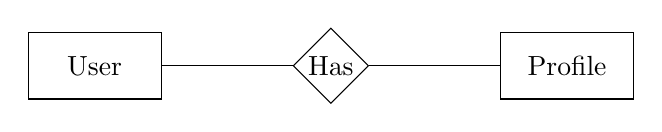
\begin{tikzpicture}[node distance = 3cm]
        \node[entity] (user) {User};
        \node[relationship] (has) [right of=user] {Has} edge (user);
        \node[entity] (profile) [right of=has] {Profile} edge (has);
    \end{tikzpicture}
\end{figure}


\begin{table}[ht]
    \centering
    \caption{Attributes of \texttt{User} model}
    \renewcommand{\arraystretch}{1.5}
    \begin{tabular}[ht]{r|l}
        \hline
        \texttt{Attribute} & Note \\
        \hline
        \hline
        \texttt{id} & primary key \\
        \hline
        \texttt{username} &  required, max length: 150 \\
        \hline
        \texttt{first\_name} &  optional, max length: 30 \\
        \hline
        \texttt{last\_name} &  optional, max length: 150 \\
        \hline
        \texttt{email} & optional\\
        \hline
        \texttt{password} & A hash of the user's password \\
        \hline
        \texttt{is\_active} & \texttt{boolean field}, indicating whether or not the user
            is active \\
        \hline
        \texttt{last\_lgoin} & \texttt{datetime field}, last login time \\
        \hline
        \texttt{data\_joined} & \texttt{datetime field}, time when the account is created \\
        \hline
    \end{tabular}
    \renewcommand{\arraystretch}{1}
\end{table}

\begin{table}[ht]
    \centering
    \caption{Attributes of \texttt{Profile} model}
    \renewcommand{\arraystretch}{1.5}
    \begin{tabular}[ht]{r|l}
        \hline
        Attribute & Note \\
        \hline
        \hline
        \texttt{user\_id} & foreign key to a \texttt{User} model instance \\
        \hline
        \texttt{role} & \texttt{integer field}, choice from 0 and 1, indicating the
            user's role \\
           & is \emph{Student} or \emph{Professor} respectively \\
        \hline
    \end{tabular}
    \renewcommand{\arraystretch}{1}
\end{table}




%-----------------------------------------------------------------------------
% Section: Course management
%-----------------------------------------------------------------------------

\subsection{Course management}

\subsubsection{Data model}

\begin{figure}[ht]
    \centering
    \caption{Data model of the course management module}
    \usetikzlibrary{er}

    \begin{tikzpicture}[scale=0.8, every node/.style={scale=0.8}, node distance = 4cm]
        \node[entity] (course) {Course};

        \node[relationship] (stu_reg) [below of=course] {Student} edge[total] (course);
        \node[entity] (stu) [left of = stu_reg] {User (Role: student)} edge[total] (stu_reg);

        \node[relationship] (instructor) [above of = course] {Instructor} edge (course);
        \node[entity] (prof) [left of = instructor] {User (Role: professor)} edge (instructor);

        \node[relationship] (ta_reg) [right of = course] {TA} edge[total] (course);
        \node[entity] (ta) [right of = ta_reg] {User} edge[total] (ta_reg);
    \end{tikzpicture}
\end{figure}

\begin{table}[ht]
    \centering
    \caption{Attributes of \texttt{Course} model}
    \renewcommand{\arraystretch}{1.5}
    \begin{tabular}[ht]{r|l}
        \hline
        \texttt{Attribute} & Note \\
        \hline
        \hline
        \texttt{id} & primary key \\
        \hline
        \texttt{department} & required, department code of the course \\ & (e.g., COMP, MATH) \\
        \hline
        \texttt{number} & required, course number \\
        \hline
        \texttt{section} & required, course section (e.g., X1) \\
        \hline
        \texttt{title} & require, course title \\
        \hline
        \texttt{semester} & required, semester of the course (e.g., Winter, Fall) \\
        \hline
        \texttt{start\_time} & required, \texttt{date} field, date the course
            becomes available to \\ & students \\
        \hline
        \texttt{end\_time} & required, \texttt{date} field, date the course ends \\
        \hline
        \texttt{visible\_after\_end} & required, \texttt{boolean} field, indicating
            whether or not to allow\\ & students access the course after it ends \\

        \hline
        \hline

        \texttt{instructor} & foreign key to the instructor \\
        \hline
        \texttt{students} & many to many relationship to the students registered \\ & in the course\\
        \hline
        \texttt{TAs} & many to many relationship to the TAs registered \\ & in the course \\

        \hline
        \hline

        \texttt{repo\_name} & optional, the name of the remote \emph{GitLab}
            repository \\ & in 
            which programming assignment source code files \\ & are stored \\
        \hline
        \hline

        \texttt{constraints} & 
            1. combination of fields
                \texttt{department},
                \texttt{number},
                \texttt{section}, \\ &
                \hspace{1.3em}\texttt{year},
                \texttt{semester} must be unique \\
            & 2. role of the \texttt{instructor} must be \emph{Professor} \\
            & 3. role of the each of the \texttt{students} must be \emph{Student} \\
        \hline
    \end{tabular}
    \renewcommand{\arraystretch}{1}
    
\end{table}





%-----------------------------------------------------------------------------
% Section: User authentication
%-----------------------------------------------------------------------------
